\section{结果}

\subsection{5.1 集中度：537 人与 108 人}

度数分布的表征量为：基尼系数（全图）0.8199，（仅带边顶点）0.6805；
平均度数全体 3.715、带边顶点 6.589；最大度数 113。
表 \ref{tab:degree} 与图 \ref{fig:deg} 是同一件事的两种读法。

\begin{table}[!t]
\centering
\caption{度数直方图（0--12 为逐度计数；13 及以上另立汇总桶，桶名 $\ge$13 不与前十三桶共名）}
\label{tab:degree}
\small
\begin{tabular}{cc}
\toprule
度数 & 人数 \\
\midrule
0 & 537 \\
1 & 343 \\
2 & 92 \\
3 & 42 \\
4 & 21 \\
5 & 16 \\
\addlinespace
6 & 13 \\
7 & 12 \\
8 & 7 \\
9 & 6 \\
10 & 7 \\
11 & 8 \\
\addlinespace
12 & 8 \\
$\ge$13 & 119 \\
最大 & 113 \\
\bottomrule
\end{tabular}
\end{table}

表 \ref{tab:degree} 的两个数最要紧：537 人度数为 0，占全部人物的 43.6\%；
另外那 694 个带边顶点里，我们把度数排序前一百的人（共 108 人，
因为第 100 名处有并列，不是 100 人整）拎出来——
这 108 人合起来握有全部度数和的 65.1\%，而他们自己只占全部人物的 8.8\%。
单人（最大度数 113）就占全部度数和的 2.5\%。
两个基尼不相等（0.8199 对 0.6805）：把 537 个孤立点并进来，
集中度读数比只看有边的人更高。这不是矛盾，是口径差，
本篇第 4.2 节已明示不许把这两个数混读。

\begin{figure}[!t]
\centering
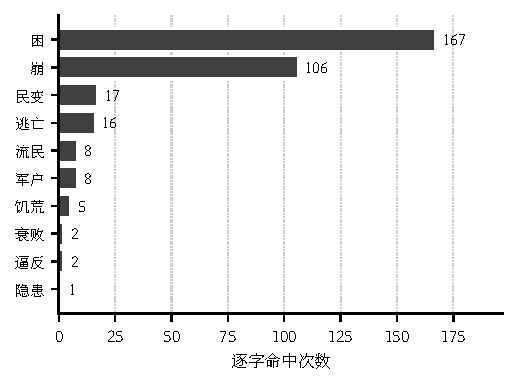
\includegraphics[width=\columnwidth]{fig_systems_1.pdf}
\caption{图 1 度数直方图：0 度 537 人，1 度 343 人，2 度 92 人，
3 度 42 人，此后逐度降到个位数，13 及以上汇总为 $\geq$13 桶共 119 人（9.7\%）。}
\label{fig:deg}
\end{figure}

\subsection{5.2 分布形状：这一条本篇负报，不主张幂律}

表 \ref{tab:alpha} 是六个切点上的 Hill 估计。

\begin{table}[!t]
\centering
\caption{Hill 尾指数随 $x_{\min}$ 的漂移（尾样本量一并列出）}
\label{tab:alpha}
\small
\begin{tabular}{crr}
\toprule
$x_{\min}$ & $\hat\alpha$ & 尾样本量 \\
\midrule
2 & 1.824 & 351 \\
3 & 1.806 & 259 \\
5 & 1.912 & 196 \\
8 & 2.142 & 155 \\
10 & 2.374 & 142 \\
15 & 2.777 & 98 \\
\bottomrule
\end{tabular}
\end{table}

$\hat\alpha$ 不是稳在一个值上：最低 1.806（$x_{\min}=3$）、最高 2.777（$x_{\min}=15$），
极差 0.971。而且它的移动方向是单调的——切点抬得越高，估计出的指数越大——
这说明看到的不是"一条稳健的幂律在不同切点上的误差"，
而是这条尾本身在 2 到 15 这一段里就不是一条直线。
按 \citet{clauset2009} 的判据，这两个条件（估计不随 xmin 漂移、尾样本足够）
在本篇都不满足：$x_{\min}=10$ 时尾样本只有 142 条。
\textbf{因此本篇不主张这批度数服从幂律，也不使用"无标度网络"这个标签描述它。}
这不是把工具扔掉：是把"复杂"从形容词降成两个还站得住的量——
基尼系数 0.8199 与最大连通块占比，下面两节就是它们。

\subsection{5.3 连通性：图是连通的，人物不是}

带边顶点 741 个，连通块 18 个（前 12 个规模的排序为 703, 4, 3, 3, 2, 2, 2, 2, 2, 2, 2, 2）。
最大块 703 点，占带边顶点的 94.9\%，占全部人物的 57.1\%。
也就是说：只要一个人至少出现在一条关系里，他有 94.9\% 的概率和朱棣、崇祯、
李自成在同一块里；但把这 1231 人整体看作一个总体而言，
这张网只罩住了其中的 57.1\%，剩下 43.6\%（即那 537 人）根本不在这张网上。
其余 17 个块加在一起只有 38 个带边顶点落在最大块之外。
这一条是本篇对"涌现"最实的一处读数：宏观的连通是真的，
但宏观的覆盖是假的——图是一整块，人物不是一整块。

\subsection{5.4 时间：不是均匀增长}

1006 件带年份事件落在 218 个年份上（1328—1645），
年均 4.615 件、标准差 5.353、变异系数 1.16、按年基尼 0.5069。
图 \ref{fig:ts} 是十年桶。三个峰很清楚：
1590 年代（101 件）、1630 年代（84 件）、1400 年代（68 件）；
单年峰值是 1519 年与 1593 年（各 32 件）与 1449 年（31 件，土木堡之变）。
按年基尼 0.5069 意味着事件量在年份之间分配得极不均匀：
一半左右的年几乎没有事件，另外一些年份一压进来就是几十件。
这不是一条平缓的兴衰曲线，是一组脉冲。

\begin{figure}[!t]
\centering
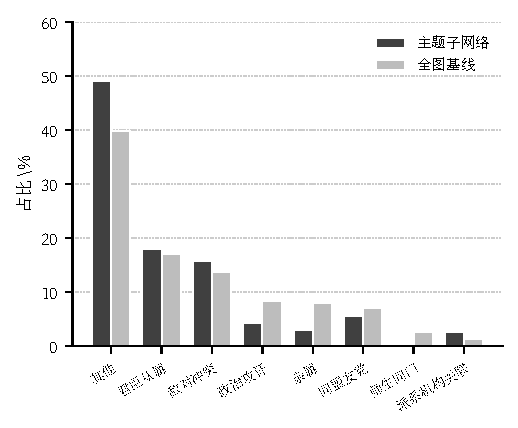
\includegraphics[width=\columnwidth]{fig_systems_2.pdf}
\caption{图 2 十年桶的事件数（1328—1645）。三个峰在 1590 年代、1630 年代、1400 年代。}
\label{fig:ts}
\end{figure}

\subsection{5.5 时期迁移：危机换了类，不是同一个危机的延续}

表 \ref{tab:shift} 是三期的事件类别占比，图 \ref{fig:shift} 是它的形状。

\begin{table}[!t]
\centering
\caption{三个时期的事件类别占比（%）；每列一行，P1 = 1368--1499（301 件），
P2 = 1500--1599（473 件），P3 = 1600--1662（186 件）}
\label{tab:shift}
\small
\begin{tabular}{lrrr}
\toprule
类别 & P1 & P2 & P3 \\
\midrule
军事战争 & 28.9 & 21.8 & 40.9 \\
政治斗争 & 33.9 & 40.8 & 21.5 \\
人事任免 & 2.3 & 10.4 & 7.0 \\
案件刑狱 & 8.0 & 3.4 & 11.3 \\
\bottomrule
\end{tabular}
\end{table}

卡方独立性检验给出 $\chi^{2}=129.05$、自由度 20、p 值小于 $10^{-6}$，
效应量 Cramér's V=0.259。这两项合起来的意思是：
时期与事件类别不是独立的（p 极小），但关联强度只到中等（V=0.259 不到 0.3），
所以本篇报的迁移是"位置明显移动，但不是类别被彻底重写"。
方向最清楚的一项是两条相反的运动：
军事战争 28.9 $\to$ 21.8 $\to$ 40.9，
政治斗争 33.9 $\to$ 40.8 $\to$ 21.5。
也就是说，第三期（1600--1662）里战场重新压上来，
而前两期一路上升的政治斗争占比在第三期掉下去
——后一段不是同一场危机的延续，是另一类事件补位。
三期各自牵涉到的参与人物数为 283、403、209 人（按事件 participants 去重计），
人数最多的中段（P2）与占比最动的三期并不重合，
说明占比迁移不完全由"哪期人多"驱动。

\begin{figure}[!t]
\centering
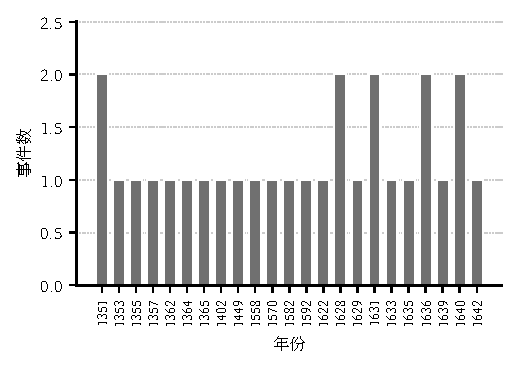
\includegraphics[width=\columnwidth]{fig_systems_3.pdf}
\caption{图 3 四类事件在三期的占比（%）。军事战争与政治斗争在 P3 方向相反。}
\label{fig:shift}
\end{figure}

\subsection{5.6 四个量落成的形状}

把第 5.1--5.5 节合起来，"兴衰是涌现"这句话在本篇数据上能落成：
一个 43.6\% 的人不在网上的网（5.1、5.3），
一个不成立的无标度标签（5.2），
一片脉冲式而非平缓的时间（5.4），
以及一次中期—末期的危机换类（5.5）。
这四件里没有一件能单独叫"崩塌的涌现"；
它们合起来也只能说明，这部叙事在抽取之后长成了这么一张图。

以上各项均可在 \texttt{.dump/}\_stats\_systems.json 中逐项回溯。
